%!TEX root = ../Security&NetworkManagement.tex
\chapter{VPNs}
Una VPN (Virtual Private Network) è una rete di telecomunicazioni privata, instaurata tra soggetti che utilizzano, come tecnologia di trasporto, un protocollo di trasmissione pubblico e condiviso, come ad esempio la rete Internet. Un azienda, con più sedi, può aver bisogno di offrire, ai suoi clienti o ai dipendenti, un servizio equivalente a quello ottenibile tramite l'uso di un'infrastruttura privata. 

I primi esempi di Private Network erano le linee dedicate, tipi di connessione realizzate fisicamente tramite un \textquotedblleft cavo" ad essa riservato. Esse fornivano una rete realmente privata e abbastanza sicura. Il problema risiedeva in primis nel costo e nella configurazione. La versione moderna di linea dedicata è il canale ATM (Asynchronous Transfer Mode), un protocollo di rete che implementa un modo di trasferimento a commutazione di circuito virtuale e trasmissione di cella, incapsulando i dati in unità, dette celle, anziché in pacchetti a lunghezza variabile come avviene invece nelle reti a commutazione di pacchetto (es. IPv4). Anche qui gli svantaggi erano i costi, e la cattiva integrazione con il protocollo IP.

Lo scopo delle reti VPN è quello di offrire alle aziende le stesse possibilità delle linee private a noleggio, ma sfruttando reti condivise pubbliche: si può vedere dunque una VPN come l'estensione a livello geografico di una rete locale privata aziendale sicura che colleghi tra loro siti interni all'azienda stessa variamente dislocati su un ampio territorio. Le VPN hanno un bassissimo costo (poichè sfruttano Internet) e hanno un ottima integrazione con il livello IP (vengono anche detto VPN IP-based). Non hanno però un QoS prevedibile e sono in teoria più insicure. Per realizzare, dunque, una VPN sicura ho bisogno di risolvere alcuni problemi legati all'IP:
\begin{enumerate}
\item Sicurezza (sniffing, etc.) $\rightarrow$ Criptazione (IPsec)
\item Routing Dinamico $\rightarrow$ VPN Layer 2/3
\item QoS incerta $\rightarrow$ IntServ/DiffServ o MPLS
\item Scarsità degli indirizzi $\rightarrow$ NAT o IPv6
\end{enumerate}

\subsubsection{IPsec}
IPsec (IP secure) è uno standard in grado di ottenere connessioni sicure su reti IP. La sicurezza viene raggiunta attraverso funzionalità di autenticazione, cifratura e controllo di integrità dei pacchetti IP. La capacità di fornire protezione o sicurezza viene fornita quindi a livello di rete (diversamente da HTTPS, SSL/TLS), fatto che rende questo protocollo trasparente al livello delle applicazioni che non devono quindi essere modificate. L'IPsec, insieme alle VPN, permette quindi di:
\begin{itemize}
\item Rendere sicure le comunicazione tra diversi uffici di un organizzazione 
\item Rendere sicuro l'accesso remoto via Internet 
\item Stabilire connettività intranet/extranet con partner aziendali
\item Migliorare la sicurezza nel commercio elettronico
\end{itemize}

\begin{figure}[htbp]
	\centering
	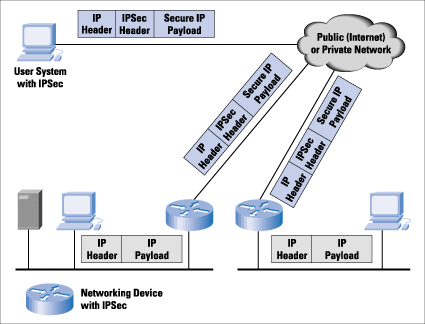
\includegraphics[scale = 0.7]{images/VPN}
	\caption{\textit{\textbf{Esempio:}} Due diversi sedi comunicano tramite un tunnel reso sicuro. Gli utenti esterni (telelavoro, roadwarrior, utenti in viaggio, etc.) accedono alla rete aziendale tramite un canale sicuro. Attraverso Internet, però, non è possibile vedere il contenuto dei pacchetti da terze parti non autorizzate.}
	\label{img:vpn-ipsec}
\end{figure}

IPsec può lavorare attraverso due protocolli:
\begin{enumerate}
\item Autenticazione e Integrità (Authentication Header, AH): Permette di autenticare il mittente e evitare attacchi “man in the middle”, ma non cripta il payload.
\item Autenticazione, Criptazione e Integrità (Encapsulating Security Payload, ESP): Autenticazione del mittente e criptazione del payload. Livello massimo di
sicurezza, ma viene “oscurato” il payload IP, quindi crea problemi per il caching, il filtering, gestione della QoS e traduzione NAT.
\end{enumerate}

Entrambi AH ed ESP hanno due \textquotedblleft modalità":
\begin{enumerate}
\item Transport Mode: L'header IP originale viene mantenuto ma bisogna ricalcolare i checksum dell'IP e TCP (Questa cosa può dar noia se si usa un NAT, vd. Capitolo 5). 
\item Tunnel Mode: L’intero pacchetto IP viene incapsulato in un nuovo pacchetto IPsec.
\end{enumerate}
\begin{figure}[htbp]
	\centering
	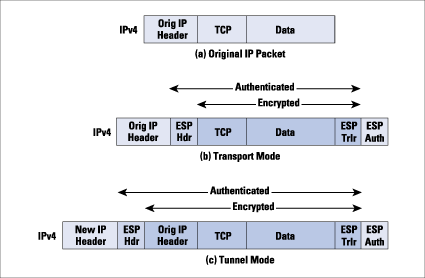
\includegraphics[scale = 0.7]{images/TransferTunnelMode}
	\caption{Modalità Transport e Tunnel Mode}
	\label{img:transporttunnel}
\end{figure}